%% **************************** Sub Test ****************************
\setcounter{Sec}{0}\setcounter{Step}{0}

\newpage
\renewcommand{\subprocid}{{\procid}-02}

\newpage
\subsection{\subprocid \ Aliveness and Functional Test}


%% Test Setup
\begin{figure}[H]
	\centering
	  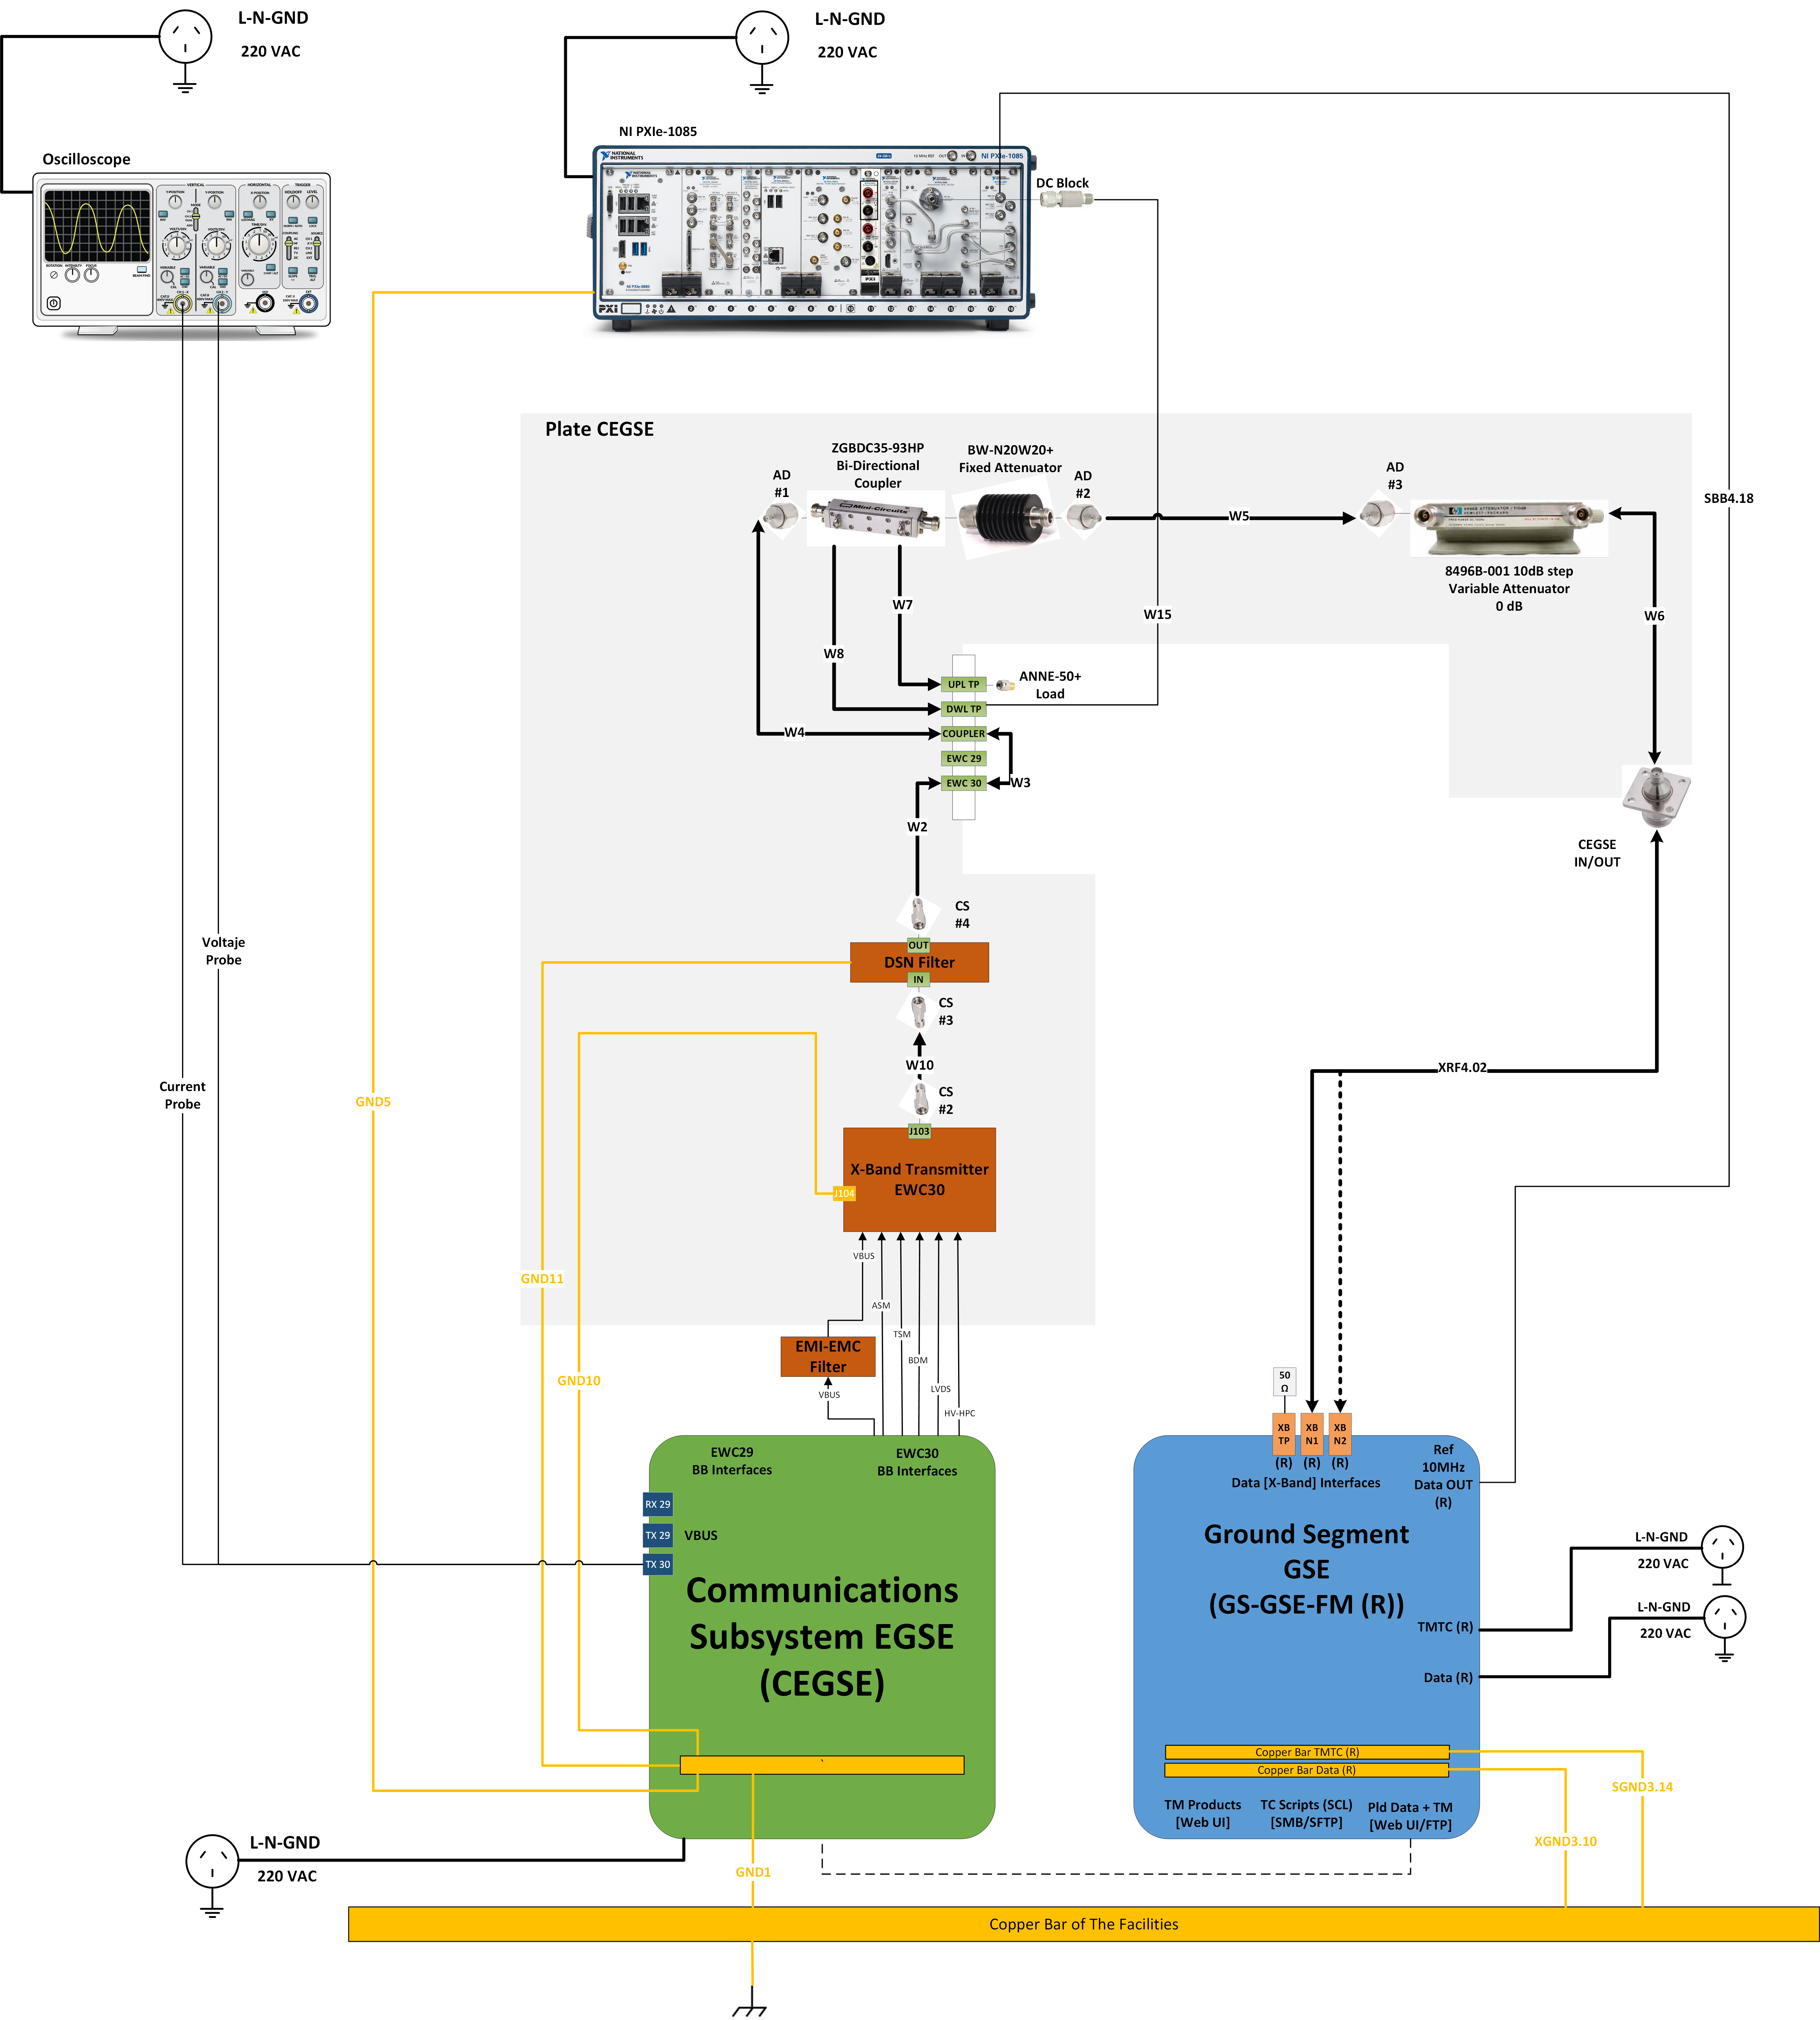
\includegraphics[width=.9\linewidth]{figuras/EWC30PXISetupB.png}  
	  \caption{Aliveness and functional test setup.}
	\label{fig:setup_xband_funcional}
	\end{figure}
\newpage
\begin{stepstable}{\subprocid{} Aliveness and Functional Test}
	\ExecutorRecord

	\SectionHeaderWithReset{Environmental temperature and humidity}
		\RegisterTempAndHumidity
		%\ConfigDatalogger

	\SectionHeaderWithReset{Preparation of GS-GSE}
		\EnableNOneInterfaceXBand{Note: Skip this step if \textbf{EWC30-FM2} is under test.}
		\EnableNTwoInterfaceXBand{Note: Skip this step if \textbf{EWC30-FM1} is under test.}
		%\VerifyConfigurationInCortexHdr
		\OpenWinCortexHDR
	
	\SectionHeaderWithReset{PXI Spectrum Analyzer connection}
		\ConnectRfCableToDwlTpPortOfCegse{W15}{}
    	\ConnectCableToDcBlock{W15}

	\SectionHeaderWithReset{Instrument configuration}
		\StartPXISpectrumA
		\configPXISpectrumA{NI-RFSA-Data-N1.tdms if EWC30-FM1 is under test}{NI-RFSA-Data-N2.tdms if EWC30-FM2 is under test}
		\ConfigPowerBandPXI{195 MHz}
		\SectionHeaderWithReset{EGSE Settings}
		%\SetCegseVariableAttenuatorTo{1 dB}{5 dB}
		\SetCegseVariableAttenuatorTo{10 dB}{0 dB}
	\SectionHeaderWithReset{CEGSE SW Initialization}
		\StartCegseSW{EWC30}{Nominal}{INIT\string_FILE\string_EWC30.ini}{}

	\SectionHeaderWithReset{DUT Power On}
		\VerifyDutAlarms{EWC-30}{}
		\TakeNoteDutTemperaturesXBand{}
		\LoadOscilloscopeConfigFile{EWC30-TX-ON.set}{}
		\PressSingleOnOscilloscope
		\TurnOnOffVbusXBand{on}{}
		\TakeScreenShotOnOscilloscope
		\MeasureInrushCurrentOn{CH1}
		\SaveOscilloscopeRawValues
		\LoadOscilloscopeConfigFile{EWC30-TX-RUN.set}{}{}
		%\SimpleExeStep{\tr{validar cooriente y potencia}}{arg2}{arg3}
		\TakeNoteOfCurrentAndVoltageOf{TX}{CH1}{CH2}{28 V}{< 282 mA}{} 
		\VerifyPowerConsumptionOf{TX}{CH1}{CH2}{P $\approx$\ 8 W@standby}
		%\LoadOscilloscopeConfigFile{EWC30-TX-RIPPLE.set}{}
	
	
	\SectionHeaderWithReset{Verify DUT Telemetry}
		\VerifyRxSecondaryVoltageRFXBand
		\VerifyRxSecondaryVoltageNUMXBand
    	\VerifyRfOutputPowerTmXBand{< 0.5}
    	\VerifyTemperature{O\string_TX\string_TEMP1}{}
    	\VerifyClkLockedStatus{OFF}
    	\VerifyMmuClkStatus{OFF}
    	\VerifyTxStatusSBand{Standby}
		%\VerifyTxStatus{stand-by}{O\string_TX\string_STATUS = 0}

	% \SectionHeaderWithReset{Preparation of GS-GSE}
	% 	\EnableNOneInterfaceXBand{Note: Skip this step if \textbf{EWC30-FM2} is under test.}
	% 	\EnableNTwoInterfaceXBand{Note: Skip this step if \textbf{EWC30-FM1} is under test.}
	% 	%\VerifyConfigurationInCortexHdr
	% 	\OpenWinCortexHDR
		
		%%%%%%%%%%%%%%%%%%%%%%%%%%%%%%%%%%%%%%%%%%%%%%%%%%%%%%%%%%%%%%%%%%%%%%%%%%%%%%%%%%%%%%%%%%%%%%%%%%%%%%%%%%%
		% Medicioens de corriente  de ripple
		%%%%%%%%%%%%%%%%%%%%%%%%%%%%%%%%%%%%%%%%%%%%%%%%%%%%%%%%%%%%%%%%%%%%%%%%%%%%%%%%%%%%%%%%%%%%%%%%%%%%%%%%%%%
	\SectionHeaderWithReset{File generation for data transmission}
		\GenerateDownlinkFileXBand{1330000 ($\approx$180 seconds)}{1330000}{Data-885840\_120s\_VCh01\_payload.bin}{}
	\SectionHeaderWithReset{Ripple voltage and current measurement}
	\VerifyTemperature{O\string_TX\string_TEMP1}{}
		\SendGeneratedFileXBand{I\_STBY\_2\_OPE\_M}{main}
		\VerifyTxStatusXBand{Modulation}
		%\CheckLookCortexHDR
    	%\StartIngestionInCortexHdr
		\VerifyClkLockedStatus{ON}
		\VerifyRfOutputPowerTmXBand{$\approx$ 3.2}
  		\TakeNoteOfCurrentAndVoltageOf{TX}{CH1}{CH2}{28\ V}{$\approx$ \ValueCurrentDUTTX A}{\notaCorrienteEstimada}
		\LoadOscilloscopeConfigFile{EWC30-TX-RIPPLE.set}{}
		\adquicicionOSCStop
		\TakeScreenShotOnOscilloscope
		\SaveOscilloscopeRawValues
		\adquicicionOSCStart
		\ChangeTimeConf
		\adquicicionOSCStop
		\TakeScreenShotOnOscilloscope
		\SaveOscilloscopeRawValues
		\TakeNoteOfCurrentAndVoltageRippleOf{TX}{CH1}{CH2}{\ValueVRipple}{\ValueIRippleADHBoxToFilter}

		\SectionHeaderWithReset{Ripple  current measurement}
		\ConnectMeasurementProbeBetweenFilterAndDUT

		\LoadOscilloscopeConfigFile{EWC30-TX-RIPPLE.set}{}
		\adquicicionOSCStop
		\TakeScreenShotOnOscilloscope
		\SaveOscilloscopeRawValues
		\adquicicionOSCStart
		\ChangeTimeConf
		\adquicicionOSCStop
		\TakeScreenShotOnOscilloscope
		\SaveOscilloscopeRawValues
		\TakeNoteOfCurrent{TX}{CH1}{\ValueIRippleDUTToFilter}
		%\adquicicionOSCStart
		\ConnectMeasurementProbesToAdHocBoxForXBand
		\LoadOscilloscopeConfigFile{EWC30-TX-RUN.set}{}{}
		%\WaitUntilTxFinishedOnCegse
		%\StopIngestonInCortexHdr
		\ChangeTxStatusTo{I\string_OPE\string_2\string_STBY\string_M }{standby}
		\VerifyTxStatusXBand{Standby}
		\StopXB

	%%%%%%%%%%%%%%%%%%%%%%%%%%%%%%%%%%%%%%%%%%%%%%%%%%%%%%%%%%%%%%%%%%%%%%%%%%%%%%%%%%%%%%%%%%%%%%%%%%%%%%%%%%%
    %%%%%%%%%%%%%%%%%%%%%%%%%%%%%%%%%%%%%%%%%%%%%%%%%%%%%%%%%%%%%%%%%%%%%%%%%%%%%%%%%%%%%%%%%%%%%%%%%%%%%%%%%%%

   %\SectionHeaderWithReset{File generation for data transmission}
   %   \GenerateDownlinkFileXBand{1000000 ($\approx$135 seconds)}{1000000}{Data-885840\_120s\_VCh01\_payload.bin}{}

	\SectionHeaderWithReset{RF measurements with the PXI Spectrum Analyzer and Data Downlink test}
   		\VerifyTemperature{O\string_TX\string_TEMP1}{}
		\SendGeneratedFileXBand{I\_STBY\_2\_OPE\_R}{redundant}
		\VerifyTxStatusXBand{Modulation}
		\CheckLookCortexHDR
    	\StartIngestionInCortexHdr
		\VerifyRxSecondaryVoltageRFXBand % mezcla
		\VerifyRxSecondaryVoltageNUMXBand % mezcla
		\VerifyClkLockedStatus{ON}
		\VerifyMmuClkStatus{ON} % de mezcla
		%\VerifyRfOutputPowerTmXBand{$\approx$ 3.2} % estaba antes
		%\LoadOscilloscopeConfigFile{EWC30-TX-RIPPLE.set}{}{}
		%\adquicicionOSCStop
		%\TakeScreenShotOnOscilloscope
		%\SaveOscilloscopeRawValues
		%\adquicicionOSCStart
		%\ChangeTimeConf
		%\adquicicionOSCStop
		%\TakeScreenShotOnOscilloscope
		%\SaveOscilloscopeRawValues
		%\TakeNoteOfCurrentAndVoltageRippleOf{TX}{CH1}{CH2}{542\ mVpp}{750\ mApp}
		%\adquicicionOSCStart
        
		\VerifyRfOutputPowerTmXBand{$\approx$ 3.2} % de mezcla
		\TakeNoteOfCurrentAndVoltageOf{TX}{CH1}{CH2}{28\ V}{$\approx$ \ValueCurrentDUTTX A}{\notaCorrienteEstimada}
		\MeasureCarrierPowerModUsingPxi{40\ }{1} % de mezcla
		\TakeScreenShotOnPxi  % de mezcla
		\ConfigBandWidthPXI   % de mezcla
		\MeasureOccupiedBandwidthUsingPxi{205} % de mezcla
		\TakeScreenShotOnPxi  % de mezcla



		\WaitUntilTxFinishedOnCegse
		\StopIngestonInCortexHdr
		\MeasureLOLeakageUsingPxi % de mezcla
		\ChangeTxStatusTo{I\string_OPE\string_2\string_STBY\string_R }{standby} % de mezcla
		%\ChangeTxStatusTo{I\string_OPE\string_2\string_STBY\string_M }{standby}
		\VerifyTxStatusXBand{Standby} % de mezcla
		%\VerifyTxStatusXBand{Standby}

	\SectionHeaderWithReset{Verify received data}
		\VerifyNumberOfIdlesFramesReceivedInCortexHdr
		\VerifyNumberOfFramesReceivedVCOneInCortexHdr{1}{885840}
		\StartDataRFFlow{1800}
		\WaitForDataFlowExecution
		\LoginToCCM
		\GoToProductsOnCCM
		\FindXBandProductOnCCM
		\DownloadIdentifiedProductFromCCM{}
		\RemoveTransportLayer{X Band}{885840}
		\CompareDownlinkPayloadFiles{EWC30}{\fileXbCompare}
		
    % \SectionHeaderWithReset{RF measurements with the PXI Spectrum Analyzer}
	% 	\VerifyTemperature{O\string_TX\string_TEMP1}{}
	% 	\SendGeneratedFileXBand{I\_STBY\_2\_OPE\_R}{redundant}
	% 	\VerifyTxStatusXBand{Modulation}
	% 	\CheckLookCortexHDR
	% 	\VerifyRxSecondaryVoltageRFXBand
	% 	\VerifyRxSecondaryVoltageNUMXBand
	% 	\VerifyClkLockedStatus{ON}
	% 	\VerifyMmuClkStatus{ON}
	% 	\VerifyRfOutputPowerTmXBand{$\approx$ 3.2}
	% 	\MeasureCarrierPowerModUsingPxi{40\ }{1}
	% 	\TakeScreenShotOnPxi 
	% 	\ConfigBandWidthPXI
	% 	\MeasureOccupiedBandwidthUsingPxi{205}
	% 	\TakeScreenShotOnPxi 
	% 	\WaitUntilTxFinishedOnCegse
	% 	\MeasureLOLeakageUsingPxi
	% 	\ChangeTxStatusTo{I\string_OPE\string_2\string_STBY\string_R }{standby}
	% 	\VerifyTxStatusXBand{Standby}

	\SectionHeaderWithReset{DUT Turn Off}
		\LoadOscilloscopeConfigFile{EWC30-TX-OFF.set}{}
		\PressSingleOnOscilloscope
		\TurnOnOffVbusXBand{off}{}
		\TakeScreenShotOnOscilloscope
		\MeasurePowerDownCurrentOn{CH1}
		\SaveOscilloscopeRawValues
	
	\SectionHeaderWithReset{CEGSE SW Shutdown}
		\StopCegseSW{}

	\SectionHeaderWithReset{Collect Evidences}
		\CopyCegseLogsForEvicences{\subprocid}{}
		\CopyOscilloscopeScreenShotsForEvidences
		\GetTempAndHumidityFromDatalogger
		%\ConnectPendriveTo{oscilloscope}

	\SectionHeaderWithReset{Final Steps}
		\SetReduntanSideOnXbmaDisableMandC
		\RegisterTempAndHumidity
		\DisconnectRfCableFromDwlTpOfCegse{W15}{}
		\DisconnectCableFromDcBlock{W15}{} 
		\ClosePXISA
		%\ClosePXIM 

\end{stepstable}
\begin{longtable}{|p{17.0cm}|}
	\endfirsthead
	\endfoot
	\caption{Procedure \subprocid \ table.} \label{tb:proc:018-02}
\end{longtable}
